\documentclass[border=3pt]{standalone}
% Preâmbulo compartilhado pelos diagramas TikZ da aula 9 de IHC (Princípios e Diretrizes)
\usepackage[T1]{fontenc}
\usepackage[utf8]{inputenc}
\usepackage{lmodern}
\usepackage{amsmath}
\usepackage{xcolor}
\usepackage{tikz}
\usetikzlibrary{arrows.meta,angles,quotes,decorations.pathmorphing,decorations.pathreplacing,calc,
                positioning,shapes.geometric,shapes.misc,backgrounds,fit,
                math}

% Paleta (mesma dos SVGs originais)
% Paleta da disciplina de IHC: acento roxo (#755099), da capa do livro.
% (o nome "dblue" é mantido para não alterar todos os diagramas)
\definecolor{dblue}{HTML}{755099}
\definecolor{dorange}{HTML}{B3541E}
\definecolor{dgreen}{HTML}{4A7C59}
\definecolor{dred}{HTML}{9C4B4B}
\definecolor{dcream}{HTML}{F4F1EA}
\definecolor{dshade}{HTML}{DDD7C9}

% Função gaussiana (não normalizada por padrão de escala visual)
\pgfmathdeclarefunction{gauss}{3}{%
  \pgfmathparse{1/(#3*sqrt(2*pi))*exp(-((#1-#2)^2)/(2*#3^2))}%
}

% Estilos comuns (prefixo d... para não colidir com chaves internas do pgf)
\tikzset{
  >={Stealth[length=2mm]},
  dguide/.style={gray!55, dashed, line width=0.4pt},
  daxis/.style={gray!60, line width=0.7pt, ->},
  dbody/.style={fill=black!3, draw=black!80, line width=1pt},
  dacc/.style={draw=dblue, line width=1pt},
  dlbl/.style={black!55, font=\small},
  dsub/.style={black!45, font=\footnotesize},
  dstate/.style={circle, draw=black!80, fill=dcream, line width=1pt,
                 minimum size=17mm, font=\large, inner sep=1pt},
  dobs/.style={circle, draw=black!80, fill=dshade, line width=1pt,
               minimum size=14mm, font=\large, inner sep=1pt},
  dbox/.style={rounded corners=2pt, draw=black!80, fill=dcream, line width=1pt,
               align=center, inner sep=6pt},
  dop/.style={circle, draw=black!80, fill=white, line width=1pt,
              minimum size=6mm, inner sep=0pt, font=\small},
  dtrans/.style={->, dblue, line width=1pt},
  dmeas/.style={->, dorange, line width=1pt},
  dcurve/.style={line width=1pt, dblue},
  dcurveb/.style={line width=1.4pt, dorange},
}

\begin{document}
\hyphenpenalty=10000 \exhyphenpenalty=10000 \tolerance=9999 \emergencystretch=3em
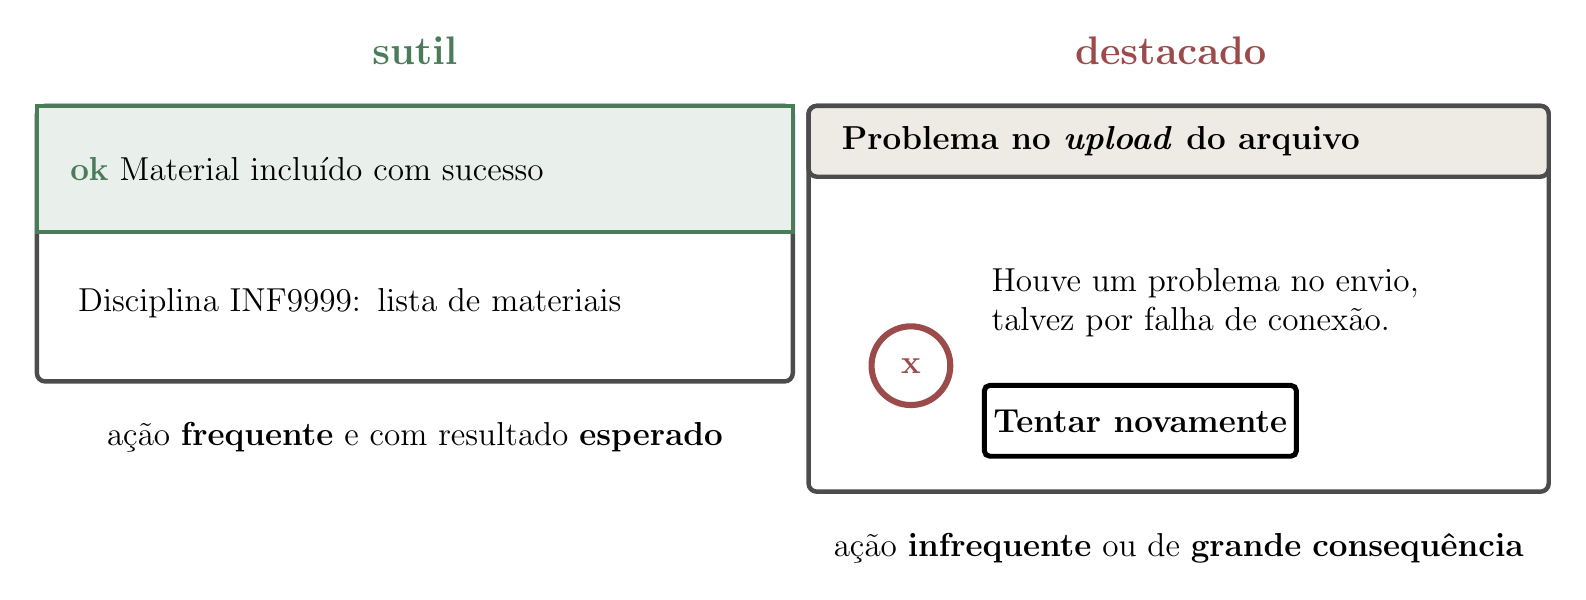
\begin{tikzpicture}[x=1cm,y=1cm]
\tikzset{d/.style={draw=black!70, line width=1.6pt, fill=white, rounded corners=3pt}}
\node[font=\Large\bfseries, dgreen] at (4.8,7.6) {sutil};
\draw[d] (0,3.4) rectangle (9.6,6.9); 
\draw[line width=1.6pt, draw=dgreen, fill=dgreen!12] (0,5.3) rectangle (9.6,6.9);
\node[font=\large, anchor=west, text width=9cm] at (0.3,6.1) {\textbf{\textcolor{dgreen}{ok}}\ Material incluído com sucesso};
\node[font=\large, anchor=west, text width=9cm] at (0.4,4.4) {Disciplina INF9999: lista de materiais};
\node[font=\large, text width=9.6cm, align=center, anchor=north] at (4.8,3.0) {ação \textbf{frequente} e com resultado \textbf{esperado}};
\node[font=\Large\bfseries, dred] at (14.4,7.6) {destacado};
\draw[d] (9.8,2.0) rectangle (19.2,6.9); \draw[d, fill=dshade!50] (9.8,6.0) rectangle (19.2,6.9);
\node[font=\large\bfseries, anchor=west] at (10.1,6.45) {Problema no \emph{upload} do arquivo};
\draw[line width=2.2pt, draw=dred] (11.1,3.6) circle (0.5); \node[font=\large\bfseries, dred] at (11.1,3.6) {x};
\node[font=\large, anchor=west, text width=6.6cm] at (12.0,4.4) {Houve um problema no envio, talvez por falha de conexão.};
\node[font=\large\bfseries, anchor=west, draw=black, line width=1.8pt, rounded corners=2pt, minimum height=0.9cm] at (12.0,2.9) {Tentar novamente};
\node[font=\large, text width=9.4cm, align=center, anchor=north] at (14.5,1.6) {ação \textbf{infrequente} ou de \textbf{grande consequência}};
\end{tikzpicture}
\end{document}
